% \section{Some Other Distributions}

% In this section, we introduce several other important probability distributions that arise in various contexts.

% \subsection{Geometric Distribution}

% The geometric distribution gives the number of trials until the first success in a sequence of Bernoulli trials.

% \[
% P(X = x) = (1 - p)^{x - 1} p, \quad x = 1, 2, 3, \ldots
% \]

% \textbf{Mean:} $\frac{1}{p}$ \quad
% \textbf{Variance:} $\frac{1 - p}{p^2}$

% \textbf{Example:} Probability of first success on $x$th trial with $p = 0.3$.

% \begin{center}
% \begin{tikzpicture}
% \begin{axis}[
%     ybar,
%     ymin=0,
%     ymax=0.4,
%     bar width=8pt,
%     xtick={1,2,3,4,5},
%     xlabel={$x$},
%     ylabel={$P(X = x)$},
%     title={Geometric Distribution ($p = 0.3$)}
% ]
% \addplot+[blue, fill=blue!30] coordinates {
%     (1,0.3)
%     (2,0.21)
%     (3,0.147)
%     (4,0.1029)
%     (5,0.07203)
% };
% \end{axis}
% \end{tikzpicture}
% \end{center}

% \subsection{Hypergeometric Distribution}

% The hypergeometric distribution models successes without replacement.

% \[
% P(X = x) = \frac{\binom{K}{x} \binom{N - K}{n - x}}{\binom{N}{n}}
% \]

% \textbf{Parameters:}
% \begin{itemize}
%     \item $N$: population size
%     \item $K$: number of successes in population
%     \item $n$: number of draws
%     \item $x$: number of observed successes
% \end{itemize}

% \textbf{Example:} Drawing 5 cards from a deck with 12 red cards ($N = 20$, $K = 12$, $n = 5$)

% \begin{center}
% \begin{tikzpicture}
% \begin{axis}[
%     ybar,
%     ymin=0,
%     bar width=8pt,
%     xtick={0,1,2,3,4,5},
%     xlabel={$x$},
%     ylabel={$P(X = x)$},
%     title={Hypergeometric Distribution}
% ]
% \addplot+[blue, fill=blue!30] coordinates {
%     (0,0.0004)
%     (1,0.0124)
%     (2,0.0929)
%     (3,0.2786)
%     (4,0.3967)
%     (5,0.219)
% };
% \end{axis}
% \end{tikzpicture}
% \end{center}

% \subsection{Exponential Distribution}

% The exponential distribution models the time between events in a Poisson process.

% \[
% f_X(x) = 
% \begin{cases}
% \lambda e^{-\lambda x}, & x \ge 0 \\
% 0, & \text{otherwise}
% \end{cases}
% \]

% \textbf{Mean:} $\mathbb{E}(X) = \frac{1}{\lambda}$ \quad
% \textbf{Variance:} $\text{Var}(X) = \frac{1}{\lambda^2}$

% \textbf{Example:} Lifetime of a battery with average 2 hours ($\lambda = 0.5$).

% \begin{center}
% \begin{tikzpicture}
% \begin{axis}[
%     width=10cm,
%     height=6cm,
%     domain=0:10,
%     samples=100,
%     xlabel={$x$},
%     ylabel={$f_X(x)$},
%     title={Exponential Distribution ($\lambda=0.5$)},
%     ytick=\empty
% ]
% \addplot[blue, very thick] {0.5*exp(-0.5*x)};
% \end{axis}
% \end{tikzpicture}
% \end{center}

% \subsection*{4. Student's $t$-Distribution}

% The $t$-distribution arises in estimating the mean of a normally distributed population when the sample size is small.

% \[
% f_T(t) = \frac{\Gamma\left( \frac{\nu + 1}{2} \right)}{\sqrt{\nu \pi}\,\Gamma\left( \frac{\nu}{2} \right)} \left(1 + \frac{t^2}{\nu} \right)^{-\frac{\nu + 1}{2}}
% \]

% \textbf{Mean:} $0$ \quad
% \textbf{Variance:} $\frac{\nu}{\nu - 2}$ for $\nu > 2$

% \begin{center}
% \begin{tikzpicture}
% \begin{axis}[
%     width=10cm,
%     height=6cm,
%     domain=-5:5,
%     samples=100,
%     xlabel={$t$},
%     ylabel={$f_T(t)$},
%     title={Student's $t$-Distribution ($\nu = 3$)},
%     ytick=\empty
% ]
% \addplot[blue, very thick] {0.3676 * (1 + (x^2)/3)^(-2)};
% \end{axis}
% \end{tikzpicture}
% \end{center}

% \subsection{Chi-Squared Distribution}

% The chi-squared ($\chi^2$) distribution is used in hypothesis testing and confidence intervals for variance.

% \[
% f_X(x) = \frac{1}{2^{k/2} \Gamma(k/2)} x^{k/2 - 1} e^{-x/2}, \quad x > 0
% \]

% \textbf{Mean:} $k$ \quad
% \textbf{Variance:} $2k$

% \begin{center}
% \begin{tikzpicture}
% \begin{axis}[
%     width=10cm,
%     height=6cm,
%     domain=0:10,
%     samples=100,
%     xlabel={$x$},
%     ylabel={$f_X(x)$},
%     title={Chi-Squared Distribution ($k = 3$)},
%     ytick=\empty
% ]
% \addplot[blue, very thick] {0.3989 * x^(0.5) * exp(-x/2)};
% \end{axis}
% \end{tikzpicture}
% \end{center}

% \subsection{F-Distribution}

% The F-distribution arises when comparing two sample variances, often used in Analysis of Variance (ANOVA) and hypothesis testing.

% \[
% f_X(x) = \frac{\Gamma\left(\frac{d_1 + d_2}{2} \right)}{\Gamma\left(\frac{d_1}{2} \right)\Gamma\left(\frac{d_2}{2} \right)} \left(\frac{d_1}{d_2} \right)^{d_1/2} \cdot \frac{x^{(d_1/2 - 1)}}{\left(1 + \frac{d_1 x}{d_2} \right)^{(d_1 + d_2)/2}}, \quad x > 0
% \]

% Where:

% - \( d_1 \): degrees of freedom of the numerator

% - \( d_2 \): degrees of freedom of the denominator

% \textbf{Mean:} \( \dfrac{d_2}{d_2 - 2} \), for \( d_2 > 2 \)  
% \textbf{Variance:} \( \dfrac{2 d_2^2 (d_1 + d_2 - 2)}{d_1 (d_2 - 2)^2 (d_2 - 4)} \), for \( d_2 > 4 \)

% \textbf{Example:} \( d_1 = 5, d_2 = 10 \)

% \begin{center}
% \begin{tikzpicture}
% \begin{axis}[
%     width=10cm,
%     height=6cm,
%     domain=0:5,
%     samples=100,
%     xlabel={$x$},
%     ylabel={$f_X(x)$},
%     title={F-Distribution ($d_1 = 5$, $d_2 = 10$)},
%     ytick=\empty
% ]
% % Approximated and simplified function
% \addplot[blue, very thick] {1.17 * x^(1.5) / (1 + 0.5*x)^7.5};
% \end{axis}
% \end{tikzpicture}
% \end{center}

\section{Why Do We Use Statistics?}

Statistics is a branch of mathematics that deals with the processes of \textit{collecting}, \textit{organizing}, \textit{analyzing}, \textit{interpreting}, and \textit{presenting} data. It plays a foundational role in nearly every discipline --- from economics and medicine to social sciences and engineering --- because it provides tools to make sense of data and draw meaningful conclusions.

\subsection{Understanding Large Amounts of Information}

In real-world scenarios, data is often abundant and complex. Without statistics, it would be difficult to extract useful insights from such information.

\begin{itemize}
  \item \textbf{Healthcare:} A pharmaceutical company conducts trials on thousands of patients. Statistical tools help determine whether a new drug is effective and safe by analyzing patient responses.
  \item \textbf{Economics:} Governments use statistical measures like unemployment rates, inflation, and GDP to assess the economy and guide public policy.
  \item \textbf{Education:} Schools analyze standardized test scores and graduation rates to evaluate performance and implement improvements.
\end{itemize}

\subsection{Making Informed Decisions}

Statistics enables individuals and organizations to make evidence-based decisions rather than relying on intuition or assumptions.

\textbf{Example:} A marketing team uses customer survey data to determine which product design is most preferred. Statistical analysis reveals which features are most liked and whether preferences vary across regions or demographics.

\subsection{Detecting Patterns and Relationships}

Statistics allows us to identify trends and relationships that are not immediately obvious.

\textbf{Example:} A ride-sharing company analyzes trip data and finds that demand peaks at certain hours and in specific areas. This insight enables the company to optimize driver availability.

\subsection{Summarizing Data Effectively}

Instead of examining thousands of individual data points, we use summary measures such as the mean, median, and standard deviation to describe the data succinctly.

\textbf{Example:} An HR department computes the average salary and variation across departments to assess whether pay equity exists in the organization.

\subsection{Foundation for Further Analysis}

Descriptive statistics serves as a stepping stone to inferential statistics, where predictions or decisions are made based on data samples.

\textbf{Example:} Before testing whether a new teaching method improves academic performance, a university summarizes students' scores to understand their distribution and variability.

\section{Data and Data Collection}

To perform any statistical analysis, the first step is to gather appropriate data. Understanding the types of data, their measurement scales, and collection methods is essential for choosing the right statistical tools.

\subsection{Types of Data: Qualitative vs. Quantitative}

\begin{itemize}
    \item \textbf{Qualitative (Categorical) Data:} This type of data represents categories or qualities that cannot be measured numerically. Examples include gender, eye color, or type of cuisine. These are often summarized using frequency counts or proportions.

    \item \textbf{Quantitative (Numerical) Data:} This data represents measurable quantities and is expressed in numbers. Examples include height, weight, income, and age. Quantitative data can be further classified as:
    \begin{itemize}
        \item \textit{Discrete Data:} Takes only specific values (usually integers). Example: Number of children in a family.
        \item \textit{Continuous Data:} Can take any value within a range. Example: The weight of a person.
    \end{itemize}
\end{itemize}

\subsection{Scales of Measurement}

Understanding the level of measurement is critical for selecting the appropriate statistical methods.

\begin{itemize}
    \item \textbf{Nominal Scale:} Data consists of categories with no natural order. Example: Blood type (\texttt{A}, \texttt{B}, \texttt{AB}, \texttt{O}).

    \item \textbf{Ordinal Scale:} Categories have a meaningful order, but the differences between them are not measurable. Example: Customer satisfaction (Satisfied, Neutral, Unsatisfied).

    \item \textbf{Interval Scale:} Numeric scale with meaningful differences, but no true zero point. Example: Temperature in Celsius.

    \item \textbf{Ratio Scale:} Like the interval scale, but with a meaningful zero. Ratios are interpretable. Example: Height, weight, income.
\end{itemize}

\subsection{Methods of Data Collection}

\begin{itemize}
    \item \textbf{Surveys:} Structured questionnaires or interviews used to collect data from a sample of individuals. Surveys are common in social sciences and marketing research.

    \item \textbf{Observations:} Data is collected by directly observing subjects without interference. Useful in naturalistic studies such as animal behavior or traffic patterns.

    \item \textbf{Experiments:} Involve manipulation of variables under controlled conditions to study causal effects. Common in scientific and clinical research.

    \item \textbf{Existing Records (Secondary Data):} Utilizes data already collected by other organizations or studies. Examples include census data, hospital records, or financial reports.
\end{itemize}

\subsection{Population vs. Sample}

\begin{itemize}
    \item \textbf{Population:} The entire set of individuals or items of interest. For example, all voters in a country, or all manufactured items in a factory batch.

    \item \textbf{Sample:} A subset selected from the population for analysis. Since studying the whole population is often impractical, a representative sample is used to draw conclusions.
\end{itemize}

\section{Methods of Displaying Data}

Presenting data visually helps in identifying patterns, trends, and outliers quickly and effectively. Different methods are used depending on the type and nature of the data.

\subsection{Tables}

Tables are used to organize raw or summarized data into rows and columns, making it easier to read and compare values.

\begin{table}[h!]
\centering
\begin{tabular}{|c|c|}
\hline
\textbf{Category} & \textbf{Frequency} \\
\hline
A & 12 \\
B & 8 \\
C & 15 \\
D & 5 \\
\hline
\end{tabular}
\caption{Example of a frequency table}
\end{table}

\subsection{Charts}

\begin{itemize}
    \item \textbf{Bar Charts:} Represent categorical data using rectangular bars with heights proportional to the values.

    \begin{center}
        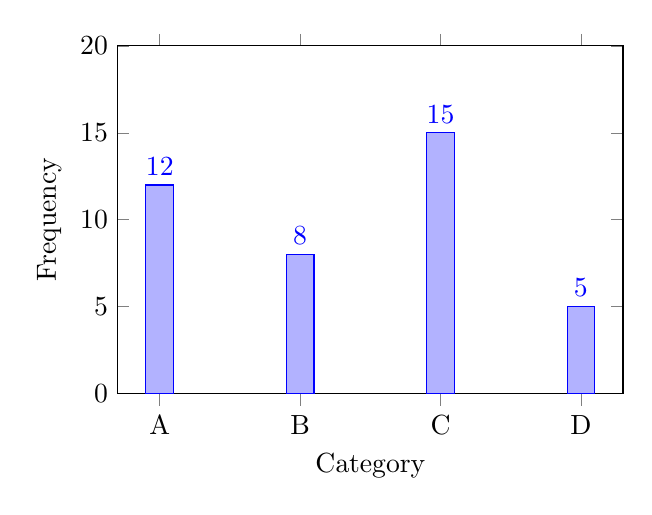
\begin{tikzpicture}
    \begin{axis}[
        ybar,
        ylabel={Frequency},
        xlabel={Category},
        symbolic x coords={A, B, C, D},
        xtick=data,
        nodes near coords,
        ymin=0, ymax=20,
        width=8cm, height=6cm
    ]
    \addplot coordinates {(A,12) (B,8) (C,15) (D,5)};
    \end{axis}
    \end{tikzpicture}
    \end{center}

    \item \textbf{Pie Charts:} Show proportions of categories as slices of a circle.

    % Pie chart requires \usepackage{pgf-pie}
    % Uncomment below if using pgf-pie
    \begin{center}
        \begin{center}
    \begin{tikzpicture}
    \pie[text=legend, radius=2]{30/A, 20/B, 40/C, 10/D}
    \end{tikzpicture}
    \end{center}
    \end{center}

    \item \textbf{Histograms:} Display the distribution of a quantitative variable by grouping data into intervals (bins).

    \begin{center}
        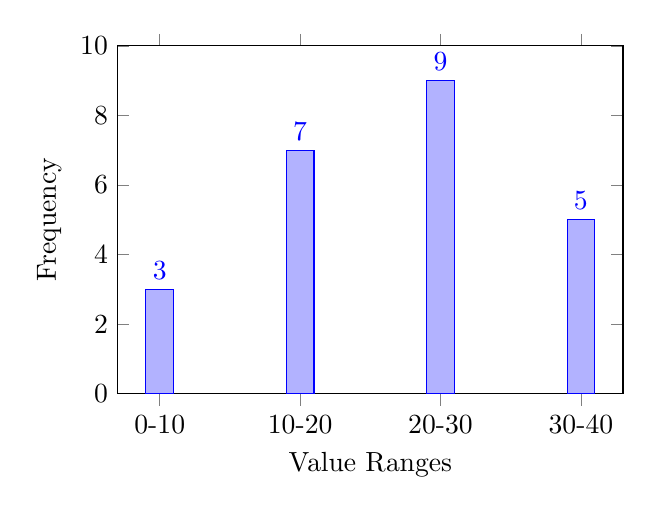
\begin{tikzpicture}
    \begin{axis}[
        ybar,
        ylabel={Frequency},
        xlabel={Value Ranges},
        symbolic x coords={0-10, 10-20, 20-30, 30-40},
        xtick=data,
        nodes near coords,
        ymin=0, ymax=10,
        width=8cm, height=6cm
    ]
    \addplot coordinates {(0-10,3) (10-20,7) (20-30,9) (30-40,5)};
    \end{axis}
    \end{tikzpicture}
    \end{center}

    \item \textbf{Box Plots:} Summarize data using the five-number summary: minimum, first quartile, median, third quartile, and maximum. Useful for detecting outliers and comparing distributions.

    % TikZ or PGFPLOTS box plots can be added with additional setup if desired
\end{itemize}

% \subsection{Stem-and-Leaf and Dot Plots}

% \begin{itemize}
%     \item \textbf{Stem-and-Leaf Plot:} Splits data into "stems" (e.g., tens) and "leaves" (e.g., units). Useful for small data sets and preserving original values.

%     \begin{center}
%     \begin{tabular}{l l}
%     \textbf{Stem} & \textbf{Leaves} \\
%     2 & 3 5 7 \\
%     3 & 1 2 4 8 \\
%     4 & 0 2 9 \\
%     \end{tabular}
%     \end{center}

%     \item \textbf{Dot Plot:} Places a dot for each data point above its corresponding value on a number line. Good for small datasets.

%     % Could add a TikZ-based dot plot here if needed
% \end{itemize}

\subsection{Time Series Plots}

A time series plot displays values over time, helping identify trends, seasonality, or irregular fluctuations.

\begin{center}
    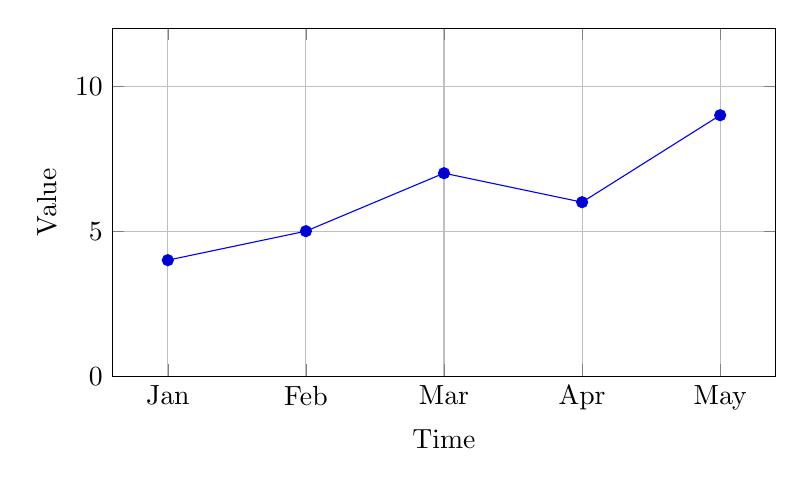
\begin{tikzpicture}
\begin{axis}[
    xlabel={Time},
    ylabel={Value},
    width=10cm,
    height=6cm,
    ymin=0, ymax=12,
    xtick={1,2,3,4,5},
    xticklabels={Jan, Feb, Mar, Apr, May},
    grid=major
]
\addplot coordinates {
    (1, 4) (2, 5) (3, 7) (4, 6) (5, 9)
};
\end{axis}
\end{tikzpicture}
\end{center}

\section{Organizing Data}

Data organization is a key step in descriptive statistics. It helps summarize large datasets to reveal patterns, facilitate comparison, and prepare for further analysis.

\subsection{Raw Data vs. Grouped Data}

\begin{itemize}
    \item \textbf{Raw data} refers to unprocessed, original observations collected directly from a source.
    \item \textbf{Grouped data} refers to data that has been organized into classes or intervals to simplify analysis.
\end{itemize}

\subsection{Frequency Tables}

Frequency tables organize data into categories or intervals and display the number of occurrences.

\subsubsection{Categorical Data}

\begin{table}[h!]
\centering
\begin{tabular}{|l|c|}
\hline
\textbf{Category} & \textbf{Frequency} \\
\hline
Red & 8 \\
Blue & 5 \\
Green & 7 \\
Yellow & 3 \\
\hline
\end{tabular}
\caption{Frequency table for categorical data}
\end{table}

\subsubsection{Numerical Data (Grouped)}

\begin{table}[!h]
\centering
\begin{tabular}{|c|c|}
\hline
\textbf{Class Interval} & \textbf{Frequency} \\
\hline
0–9   & 3 \\
10–19 & 7 \\
20–29 & 12 \\
30–39 & 6 \\
\hline
\end{tabular}
\caption{Grouped frequency table for numerical data}
\end{table}

\subsection{Relative and Cumulative Frequency}

\begin{itemize}
    \item \textbf{Relative frequency} is the proportion of each frequency relative to the total number of observations:
    \[
    \text{Relative Frequency} = \frac{\text{Frequency}}{\text{Total Frequency}}
    \]
    
    \item \textbf{Cumulative frequency} is the running total of frequencies:
    \[
    \text{Cumulative Frequency}_i = \sum_{j=1}^{i} f_j
    \]
\end{itemize}

\begin{table}[h!]
\centering
\begin{tabular}{|l|c|c|c|}
\hline
\textbf{Class} & \textbf{Frequency} & \textbf{Relative Freq.} & \textbf{Cumulative Freq.} \\
\hline
0–9   & 3  & 0.10 & 3 \\
10–19 & 7  & 0.23 & 10 \\
20–29 & 12 & 0.40 & 22 \\
30–39 & 6  & 0.20 & 28 \\
\hline
Total & 28 & 1.00 & -- \\
\hline
\end{tabular}
\caption{Frequency, relative frequency, and cumulative frequency}
\end{table}

\subsection{Histogram}

A histogram is a graphical display of frequency distribution for numerical data using adjacent bars.

\begin{center}
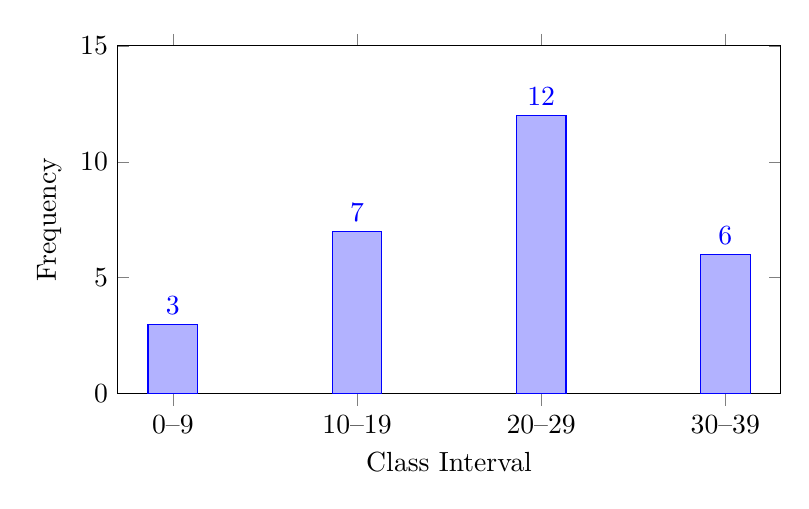
\begin{tikzpicture}
\begin{axis}[
    ybar,
    bar width=18pt,
    ylabel={Frequency},
    xlabel={Class Interval},
    symbolic x coords={0–9,10–19,20–29,30–39},
    xtick=data,
    nodes near coords,
    ymin=0, ymax=15,
    width=10cm, height=6cm
]
\addplot coordinates {(0–9,3) (10–19,7) (20–29,12) (30–39,6)};
\end{axis}
\end{tikzpicture}
\end{center}

\subsection{Frequency Polygon}

A frequency polygon connects the midpoints of the top of the bars in a histogram with straight lines.

\begin{center}
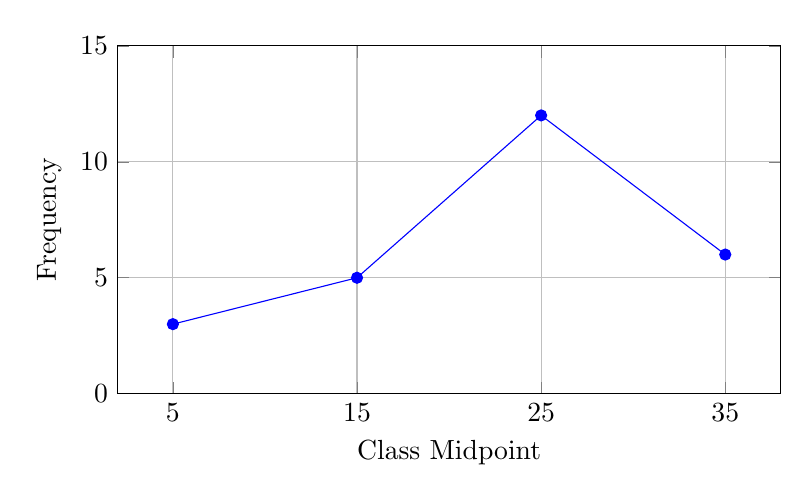
\begin{tikzpicture}
\begin{axis}[
    xlabel={Class Midpoint},
    ylabel={Frequency},
    xtick={5,15,25,35},
    xticklabels={5, 15, 25, 35},
    ymin=0, ymax=15,
    width=10cm, height=6cm,
    grid=major
]
\addplot[
    mark=*,
    color=blue
]
coordinates {
    (5,3) (15,5) (25,12) (35,6)
};
\end{axis}
\end{tikzpicture}

\subsection{Fisher Information}

Let $X_1, X_2, \dots, X_n$ be a random sample from a distribution with probability density (or mass) function $f(x; \theta)$, where $\theta$ is the parameter to be estimated. The \textbf{Fisher information} contained in a single observation $X$ is defined as
\[
I(\theta) = \mathbb{E} \left[ \left( \frac{\partial}{\partial\theta} \log f(X; \theta) \right)^2 \right]
\]
provided certain regularity conditions are met. An alternative but equivalent form is
\[
I(\theta) = -\mathbb{E} \left[ \frac{\partial^2}{\partial\theta^2} \log f(X; \theta) \right]
\]

For $n$ independent and identically distributed (i.i.d.) observations, the total Fisher information is
\[
I_n(\theta) = n \cdot I(\theta)
\]

Fisher information quantifies the amount of information the sample carries about the parameter $\theta$. More information generally leads to a more precise estimation.

\subsection{Cramér-Rao Inequality}

The \textbf{Cramér-Rao Inequality} (or Cramér-Rao Lower Bound) provides a theoretical lower bound on the variance of any unbiased estimator of a parameter $\theta$. It states that for any unbiased estimator $\hat{\theta}$ of $\theta$,
\[
\mathrm{Var}(\hat{\theta}) \geq \frac{1}{I_n(\theta)}.
\]

This bound implies that no unbiased estimator can have a variance smaller than the reciprocal of the Fisher information. If an estimator attains this bound, it is said to be \textbf{efficient}.

\subsection{Efficiency of an Estimator}

The \textbf{efficiency} of an unbiased estimator $\hat{\theta}$ is the ratio of the minimum achievable variance (given by the Cramér-Rao bound) to the actual variance of the estimator:
\[
\text{Efficiency}(\hat{\theta}) = \frac{1 / I_n(\theta)}{\mathrm{Var}(\hat{\theta})}.
\]

An estimator with efficiency equal to 1 is called \textbf{efficient}, meaning it achieves the Cramér-Rao Lower Bound. While exact efficiency is rare for finite samples, maximum likelihood estimators (MLEs) are asymptotically efficient—they approach the Cramér-Rao bound as the sample size increases.

\end{center}















